\documentclass[11pt,a4paper]{article}

\usepackage[utf8]{inputenc}
\usepackage[T1]{fontenc}
\usepackage{lmodern}
\usepackage{microtype}
\usepackage{geometry}
\geometry{margin=2.5cm}
\usepackage{amsmath, amssymb}
\usepackage{booktabs}
\usepackage{graphicx}
\usepackage{caption}
\usepackage{xcolor}
\usepackage{eurosym}
\usepackage{hyperref}
\hypersetup{colorlinks=true, urlcolor=blue!60!black, citecolor=blue!60!black,
  linkcolor=blue!60!black}
\usepackage[round,authoryear]{natbib}
\bibliographystyle{apalike}

\setlength{\parskip}{0.4em}
\setlength{\parindent}{0pt}

\title{Replicating LEAR on MIBEL through the Solar Transition: \\
Why Technical Indicators Do Not Transfer, and Why Percentage
Errors Mislead (2022--2024)}

\author{Carlo Vilches\thanks{Universitat de Barcelona --- Energy Markets Research.
Email: \texttt{cvilchce15@alumnes.ub.edu}. Data and replication code:
\url{https://github.com/cmvdata/mibel-forecasting} (folder
\texttt{paper\_forecasting/}). All inputs are public ESIOS-600 prices and ESIOS
day-ahead exogenous forecasts.}}

\date{June 2026 --- Preliminary draft}

\begin{document}
\maketitle

\begin{abstract}
\noindent We replicate the LEAR day-ahead electricity-price forecaster
\citep{lago2021} on the Iberian market (MIBEL) over 2022--2024 --- a window that
spans both the gas-crisis price regime and the onset of structural solar
saturation --- and report two cautionary findings that the replication makes
visible. The backbone result is reassuring: LEAR, recalibrated daily, beats a
seasonal-naive benchmark in every regime (relative MAE 0.45--0.57; Diebold--Mariano
$p<0.001$ throughout), with a demand-plus-wind exogenous block the best variant.
But two negative results are the contribution. First, the technical indicators of
\citet{demir2020}, helpful in their original setting, exhibit \emph{negative
transfer} to MIBEL: adding them degrades accuracy in every regime (relative MAE
worse by 4.8--9.5 points), because momentum/trend features add variance, not
signal, in a market whose price is already pinned by the demand and wind covariates
LEAR carries. Second, and more general, error \emph{metrics} diverge sharply as
solar penetration rises: the share of near-zero-price hours grows from 0.3\% (2022)
to 12.4\% (2024), and over the same span sMAPE explodes from 16\% to 51\% while the
mean absolute error actually \emph{falls} (18.3 to 14.0\,\euro/MWh). The same model
with the same skill thus looks three times worse or somewhat better depending only
on the metric, because percentage errors blow up as the denominator vanishes
\citep{hyndmankoehler2006}. We draw a concrete recommendation for forecasting
high-renewable markets and frame both findings as transferable cautions rather than
a claim to a better forecaster.

\medskip
\noindent\textbf{Keywords:} electricity price forecasting; LEAR; technical
indicators; forecast accuracy metrics; solar saturation; MIBEL.
\quad\textbf{JEL:} C53, Q47, C52.
\end{abstract}

\section{Introduction}

The LEAR model (Lasso-Estimated AutoRegressive) is a standard, strong open
benchmark for day-ahead electricity-price forecasting \citep{lago2021}. We port it
faithfully to MIBEL and evaluate it across 2022--2024, a period that is unusually
informative because it contains two distinct stresses: the 2022 gas-crisis price
regime and, by 2024, the structural solar saturation that drives Iberian
day-ahead prices to zero for an increasing fraction of hours. A faithful
replication on this period is useful in itself, but its real value here is that it
surfaces two cautions that generalise beyond MIBEL. We are explicit that this is a
replication-plus-diagnosis study, not a new forecaster: the contribution is the two
negative results, which are robust, grounded, and directly useful to practitioners.

\section{Data and method}

Prices are the OMIE day-ahead Spanish series (ESIOS indicator 600). The exogenous
regressors are ESIOS \emph{forecast} (\textit{previsi\'on}) products --- day-ahead
demand (indicator 460), wind (541) and solar (540) --- which are forecasts by
construction, not realised series, and against which the target is masked. We report
an AR-only configuration (no exogenous data at all) and a demand$+$wind
configuration; we flag in \S6 a residual caveat on the \emph{vintage} of the ESIOS
forecasts. LEAR follows \citet{lago2021}: a Lasso over calendar dummies and
price/exogenous lags, recalibrated each day on a rolling window; the benchmark is a
seasonal-naive predictor (same hour, previous similar day). Skill is the relative
MAE (rMAE $=$ model MAE / naive MAE) and significance the \citet{dieboldmariano1995}
test with a Newey--West correction (lag 23). Following \citet{lago2021} the
symmetric MAPE is the bounded form
\[
\mathrm{sMAPE}=\frac{100}{n}\sum_{t}\frac{2\,|y_t-\hat y_t|}{|y_t|+|\hat y_t|}\in[0,200],
\]
in which the only undefined points are the measure-zero set with
$|y_t|+|\hat y_t|=0$ (both exactly zero); we drop exactly those, and since LEAR's
forecast is essentially never exactly zero, no hours are effectively removed --- the
metric is computed over the full test set. We evaluate three regimes --- 2022 H2
(crisis), 2023 and 2024 (full years) --- plus the 2023--2024 pool, on
4{,}272--17{,}254 test hours each.

\section{Result 1: LEAR is robust across regimes (the backbone)}

Table~\ref{tab:lear} reports LEAR with the demand-plus-wind exogenous block, the
best-performing variant. It beats the naive benchmark decisively in every regime
(rMAE 0.45--0.57, all $p<0.001$), including the crisis. Adding a solar forecast on
top of demand and wind does \emph{not} help (rMAE marginally worse in 2023--2024),
consistent with the wind and demand forecasts already spanning most of the
predictable variation. This is a clean, reproducible replication of LEAR's known
strength; it is the platform for the two findings below, not the contribution.

\begin{table}[t]
\centering\small
\caption{LEAR (demand$+$wind) vs.\ seasonal naive, by regime. rMAE $<1$ means LEAR
beats naive; Diebold--Mariano $p$ against naive.}
\label{tab:lear}
\begin{tabular}{lrrrr}
\toprule
Regime & Test hours & MAE (\euro/MWh) & sMAPE (\%) & rMAE \\
\midrule
2022 (H2, crisis) & 4{,}272  & 18.3 & 16.1 & 0.566 \\
2023 (full year)  & 8{,}663  & 12.9 & 24.6 & 0.452 \\
2024 (full year)  & 8{,}591  & 14.0 & 51.0 & 0.511 \\
2023--2024 pooled & 17{,}254 & 13.5 & 37.8 & 0.481 \\
\midrule
\multicolumn{5}{l}{\emph{Diebold--Mariano $p<0.001$ in every row.}}\\
\bottomrule
\end{tabular}
\end{table}

\section{Result 2: technical indicators do not transfer}

\citet{demir2020} introduced financial technical indicators (EMA, Bollinger bands,
MACD, momentum, ROC, Coppock) as engineered features for electricity-price
forecasting, reporting gains in their setting. On MIBEL they exhibit clear
\emph{negative transfer}. Table~\ref{tab:ti} adds the same indicators to the
demand$+$wind LEAR: accuracy degrades in \emph{every} regime, by 4.8--9.5 points of
rMAE, and the degradation is largest in the calmer, solar-heavy 2023--2024 years.
The Lasso prunes almost all of the indicator coefficients, yet those it retains add
variance rather than signal: in a market whose day-ahead price is already pinned by
demand, wind and its own autoregressive structure, momentum/trend features ---
designed for slower, expectations-driven financial series --- have little
incremental information and hurt out-of-sample. The practical reading is that
technical indicators should not be imported into high-renewable EPF without a
market-specific transfer test.

\begin{table}[t]
\centering\small
\caption{Technical-indicator transfer: relative MAE of LEAR (demand$+$wind) without
vs.\ with the \citet{demir2020} indicators. Positive $\Delta$ $=$ accuracy lost.}
\label{tab:ti}
\begin{tabular}{lrrr}
\toprule
Regime & rMAE (base) & rMAE ($+$TI) & $\Delta$ (pts) \\
\midrule
2022 (H2, crisis) & 0.566 & 0.615 & $+4.8$ \\
2023 (full year)  & 0.452 & 0.538 & $+8.6$ \\
2024 (full year)  & 0.511 & 0.605 & $+9.5$ \\
2023--2024 pooled & 0.481 & 0.565 & $+8.4$ \\
\bottomrule
\end{tabular}
\end{table}

\section{Result 3: metrics diverge under solar saturation}

The most general finding concerns measurement. As Iberian solar capacity grows, the
day-ahead price hits (near-)zero for a rising share of hours: from 0.3\% of hours at
or below 1\,\euro/MWh in 2022 to 2.0\% in 2023 and 12.4\% in 2024 (8.9\% are exactly
zero or negative). The bounded symmetric MAPE we use (\S2) does \emph{not} divide by
zero --- the $|y_t|+|\hat y_t|=0$ set is dropped and is empty in practice --- but
that guard is exactly why the metric misleads rather than crashes. Each near-zero
hour, where $|y_t|+|\hat y_t|$ is small, contributes a term near the $200\%$ ceiling
almost regardless of the absolute error, so the \emph{average} sMAPE rises
mechanically with the \emph{count} of near-zero hours, not with forecast error
\citep{hyndmankoehler2006}. Figure~\ref{fig:div} and Table~\ref{tab:lear} show the
consequence --- holding the model fixed (LEAR demand$+$wind), sMAPE rises from 16\%
(2022) to 25\% (2023) to 51\% (2024) in lockstep with the near-zero share, while the
mean absolute error over the same span \emph{falls} from 18.3 to 14.0\,\euro/MWh and
the relative MAE is essentially flat ($\sim$0.5). The same forecaster, with the same
underlying skill, looks three times worse or modestly better depending only on
whether one reads sMAPE or MAE.

The recommendation is concrete: in high-renewable markets, and for any comparison
across years or markets with different solar penetration, accuracy must be reported
in absolute terms (MAE) and relative to a benchmark (rMAE), and percentage metrics
(MAPE, sMAPE) either dropped or restricted to non-zero-price hours with the exclusion
disclosed. A literature that ranks forecasters or markets on sMAPE is, increasingly,
ranking them on their solar share.

\begin{figure}[t]
\centering
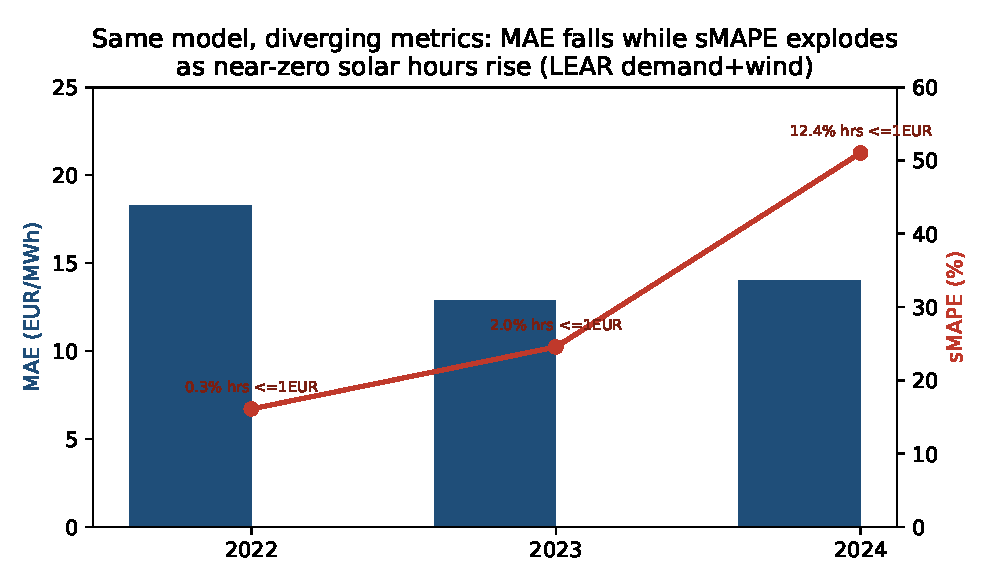
\includegraphics[width=0.74\textwidth]{fig_metric_divergence.pdf}
\caption{Same model (LEAR demand$+$wind), diverging metrics: as the share of
near-zero-price hours rises (annotated), sMAPE explodes while MAE falls.}
\label{fig:div}
\end{figure}

\section{Limitations and conclusion}

This is a replication and diagnosis, not a new model: we do not implement the deep
neural benchmark of \citet{lago2021} nor extend to the continuous intraday market,
both of which we leave for future work.

A sharper caveat concerns the \emph{vintage} of the exogenous forecasts. The demand
and wind regressors are ESIOS \textit{previsi\'on} (forecast) products, not realised
series, so the gross form of leakage --- feeding the model the realised wind and
demand it is implicitly trying to price --- is avoided by construction. But a
historical pull made in 2026 returns whatever value ESIOS currently stores for each
past timestamp, and we have \emph{not} independently confirmed that this is the
original $D\!-\!1$ forecast frozen at publication rather than a later revision. If
REE revised those forecast series ex post toward the realised outturn, the
demand$+$wind results would carry an optimistic look-ahead bias and the
Diebold--Mariano significance on that increment would be overstated. We flag this as
the first verification a referee should demand (pulling each indicator's publication
timestamp per calendar day) and report it honestly rather than asserting a clean
audit. Crucially, the backbone result does \emph{not} rest on these series: the
\textbf{AR-only} LEAR, which consumes \emph{no} exogenous data and is therefore
immune to any vintage concern, also beats the naive benchmark in every regime (rMAE
0.52--0.62, Diebold--Mariano $p<0.001$). The demand$+$wind block only sharpens an
already-significant margin.

Within that scope the conclusions are firm. LEAR transfers cleanly to
MIBEL and is robust across the crisis and the solar-transition regimes. Two
cautions, however, travel with that result and beyond it: the technical indicators
of \citet{demir2020} exhibit negative transfer and should not be adopted without a
market-specific test, and percentage error metrics become unreliable exactly as a
market decarbonises, so high-renewable EPF should be scored on absolute and
relative errors. The negative results, not the replication, are the contribution.

\bibliography{refs}

\end{document}
